\documentclass[12pt]{article}
\usepackage[margin=1in]{geometry} 
\usepackage{amsmath,amsthm,amssymb,amsfonts}
\usepackage{enumitem}
\usepackage{placeins}
\usepackage{mathtools, eucal}
\usepackage{graphicx}
\usepackage{color}
 

 
\begin{document}
 
%\renewcommand{\qedsymbol}{\filledbox}
%Good resources for looking up how to do stuff:
%Binary operators: http://www.access2science.com/latex/Binary.html
%General help: http://en.wikibooks.org/wiki/LaTeX/Mathematics
%Or just google stuff
 
\title{Homework 4 Solutions}
\author{Zheming Gao}
\maketitle

\section*{Problem 1}
\begin{enumerate}[label = (\alph*)]
\item

The graph of $P$ is the following figure.

\begin{figure}[htbp]
  \caption{Graph of $P$.}
  \centering
    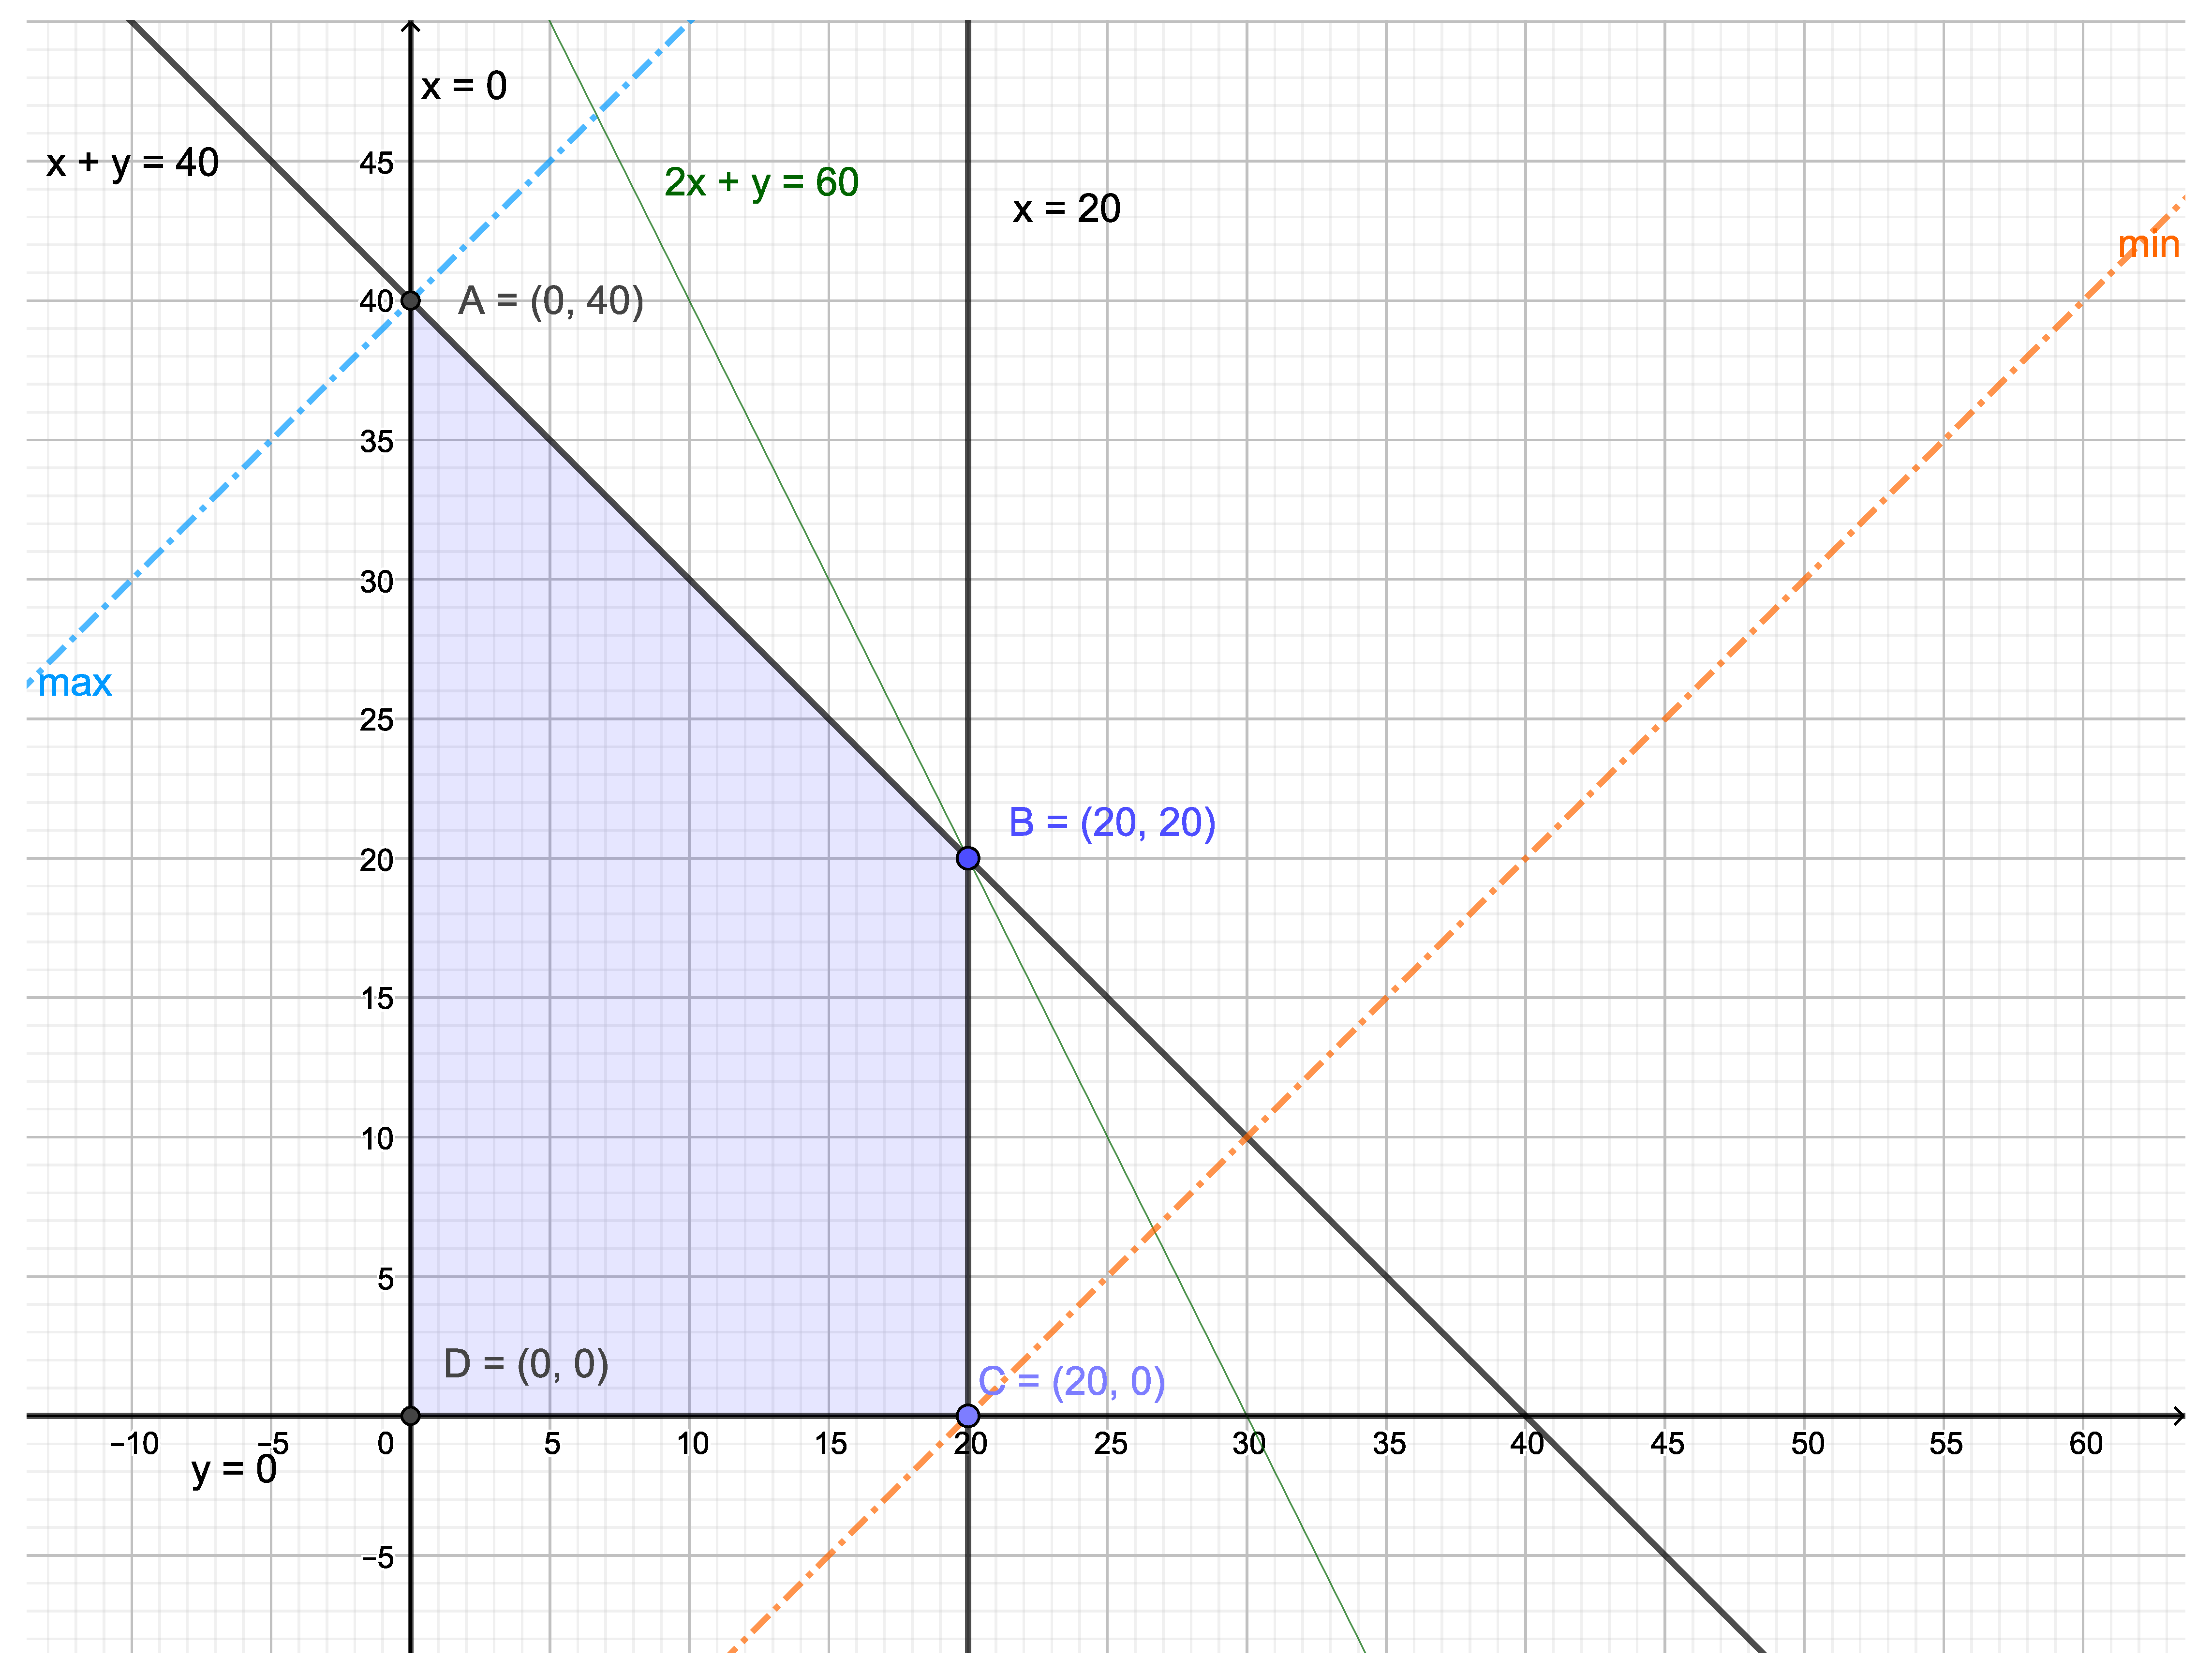
\includegraphics[width=0.5\textwidth]{2_7f.pdf}
\end{figure}

\FloatBarrier

\item

Convert $P$ to standard equality form.
$$
\left\{
\begin{aligned}
& x_1 + x_2 + a_3 & & & = 40 \\
& 2x_1 + x_2 & + a_4 & &  = 60  \\
& x_1 & & + a_5 & = 20  \\
& x_1, x_2, a_3, a_4, a_5 & & & \geqslant 0.
\end{aligned}
\right.
$$

\item [(d)\& (f)]

Basic solutions (in the form of $(x_1, x_2, a_3, a_4, a_5)$): 
$$
\begin{aligned}
&(20, 20, 0, 0, 0)  \star, \qquad (B)\\ 
&(20, 0, 20, 20, 0) \star, \qquad (C)\\ 
&(30, 0, 10, 0, -10) \\
& (40, 0, 0, -20, -20) \\ 
 & (0, 60, -20, 0, 20) \\
 & (0, 40, 0, 20, 20) \star, \qquad (A)  \\
 & (0, 0, 40, 60, 20) \star , \qquad (D)
\end{aligned}
$$



\item
Basic feasible solutions are those basic solutions with "$\star$".


\item [(e)]

$(20, 20)^T$ in $P$ is the extreme point that correspond to degenerate basic feasible solutions.



\end{enumerate}


\section*{Problem 2}

\begin{proof}

First we need to set up the problem. Let the origin LP problem have $m$ variables in it. For its standard form, let the feasible region be $\{Ax = b,  x\geqslant 0\}$ where $A\in\mathbb{R}^{m\times n}$ and $x\in \mathbb R^n$ after adding slack variables.

Now, we know that the number of positive elements in a degenerate basic feasible solution is $p$ and $p < m$. Hence, the number of zero elements in it is $n-p$. It is possible that the corresponding extreme point has all positive entries. In other words, all original variables be positive and all zero entries are on the positions of those $n-m$ slack variables. Since there are $n-p$ zero entries on $n-m$ positions, there will be $C(n-p, n-m)$ different basic feasible solutions at the same time.

Hence, this situation may happen.

\end{proof}




\section*{Problem 3}

\begin{enumerate}[label = (\alph*)]
\item 

\begin{proof}

Let $M_c$ be the convex cone generated by $M$. Then, $\forall Y\in M_c$, there exists $W\in\mathbb R^2_+$, such that $Y = MW$. Since $M = \begin{pmatrix}
1 & 0 \\
0 & 1
\end{pmatrix}$, we know that $Y = W$. Hence, $M_c = \mathbb R_+^2$.

\end{proof}

{\color{red}Attention:} Here $M_c$ is convex and it is easy to show. We will show it is convex in next part.


\item

\begin{proof}

We need to show that $M_c$ is a convex cone and it is the smallest one that contains $(1, 0)^T$ and $(0,1)^T$. 

It is clear that $(1,0)^T$ and $(0,1)^T$ are in $M_c$, since we can pick $W_1 = (1,0)^T$ and $W_2 = (0,1)^T$ from $\mathbb R^2_+$ such that $Y_1 = MW_1, Y_2 = MW_2$.

Also, use the definition and easy to show $M_c$ is a cone. $\forall \lambda \geqslant 0$, $Y\in M_c (Y = MW, W\in \mathbb R^2_+)$, $\lambda Y$ is in $M_c$ since $\lambda Y = M(\lambda W)$ and $\lambda W \in \mathbb R^2_+$.

For convexity, take $Y, Z \in M_c$, $\eta \in (0, 1)$. Let $Y= MW$, $Z = MQ$, where $W, Q\in \mathbb{R}^2_+$. Hence, $\eta Y + (1-\eta )Z = M(\eta W + (1-\eta )Z) \in M_c$ because $\eta W + (1-\eta )Z \in \mathbb{R}^2_+ $.

How to prove it is smallest? Suppose there is a convex cone $S\subset  \mathbb{R}^2$ such that contains $(1, 0)^T$ and $(0,1)^T$ but $S\subset M_c$.

Then for any $X = (x_1, x_2)^T \in M_c \setminus S $, $X = MX$(recall $M$ is the identity matrix and $X$ is also in $\mathbb R^2_+$). Since $S$ is a convex cone, $x_1(1, 0)^T + x_2 (0, 1)^T = (x_1, x_2)^T \in S$. This leads to a contradiction. In conclusion, $M$ is the smallest convex cone that contains $(1, 0)^T$ and $(0,1)^T$.

\end{proof}

\end{enumerate}



\section*{Problem 4}

\begin{enumerate}
\item[(1)]
\begin{proof}

If $d\in E$, then for any $x^0 \in P$, $x^0+\lambda d \in P$, for all $\lambda \geqslant 0$. This implies that $Ax^0 = b, x^0 \geqslant 0$, and $A(x^0 + \lambda d) = b, x^0 + \lambda d \geqslant 0$. Eliminate $Ax^0$ from the last equality and get $\lambda Ad = 0$. Since $\lambda \geqslant$, $Ad = 0$ is proved.
Also, $x^0 \geqslant 0$ and $\forall \lambda \geqslant 0$, hence $d \geqslant 0$.

Conversely, we need to show that for $d\in\mathbb R^n$, if $d \geqslant 0$ and $Ad = 0$, then $d\in E$. Take $d$ that satisfies the given condition. For any $y \in P$, $Ay = b, y \geqslant 0$. Hence, we will have $A(y + \lambda d) = b$, $\forall \lambda \geqslant 0$. Also, it is true that $y + \lambda d \geqslant 0$, due to the positiveness of $y, \lambda$ and $d$. In conclusion, $d$ is a extremal direction of $P$.
\end{proof}

\item[(2)]

\begin{proof}

We need to express $E$ in a form of set.

$$
E = \{d \in \mathbb{R}^n | y + \lambda d \in P, \forall \lambda \geqslant 0, y\in P \}.
$$

Take any $d \in E$, need to check if $\alpha d\in E$, $\forall \alpha \geqslant 0$. Actually, this is true. For any $y\in P$, $y + \lambda (\alpha d) = y + (\lambda\alpha)d \in P$ because $\lambda\alpha \geqslant 0$. Thus, $\lambda d\in E$, which proves that $E$ is a cone.

\end{proof}

\item[(3)]

\begin{proof}

Take two points $d_1, d_2 \in E$ and $\beta \in (0, 1)$. For any $y\in P, \lambda \geqslant 0$, 

$$
y + \lambda(\beta d_1 + (1-\beta)d_2) = \beta(y+\lambda d_1) + (1-\beta)(y + \lambda d_2).
$$

Let $x^1 = y + \lambda d_1$ and $x^2 = y + \lambda d_2$. Hence, the convex combination of $x^1$ and $x^2$ are in $P$ since $P$ is a convex polyhedron. This implies that $E$ is convex.

\end{proof}

\end{enumerate}












\section*{Problem 5}

\begin{enumerate}
\item [(1)]
We plot the graph of $F_3$.


\item [(2)]
$$
B = \{(x_1, x_2, x_3)^T \in \mathbb R^3 | |x_1| + |x_3| = x_2 \}.
$$



\item [(3)]

$$
I = \{(x_1, x_2, x_3)^T \in \mathbb R^3 | |x_1| + |x_3| < x_2 \}.
$$


\item [(4)]

Extreme point: $(0, 0, 0)^T$.

Vertex: $(0, 0, 0)^T$.

\item [(5)]
\begin{proof}

First, we show that $F_3$ is a cone. Take $x = (x_1, x_2, x_3)^T \in F_3$ and $\forall \lambda \geqslant 0$, check if $\lambda x \in F_3$. 

$$
|\lambda x_1| + |\lambda x_3| = \lambda |x_1| + \lambda |x_3| = \lambda (|x_1| + |x_3|) \leqslant \lambda x_2.
$$

Hence, $\lambda x$ is in $F_3$. In conclusion, $F_3$ is a cone.

Next, we need to show $F_3$ is convex. Take $x, y \in F_3$ and $\forall \eta \in (0, 1)$, $\eta x + (1- \eta) y = (\eta x_1 + (1-\eta)y_1, \eta x_2 + (1-\eta)y_2, \eta x_3 + (1-\eta)y_3)$. Use triangle inequality of absolute value and we get

$$
\begin{aligned}
|\eta x_1 + (1-\eta)y_1| + |\eta x_3 + (1-\eta)y_3| & \leqslant \eta |x_1| + (1-\eta)|y_1| + \eta |x_3| + (1-\eta)|y_3| \\
& = \eta (|x_1|+|x_3|) + (1-\eta)(|y_1|+|y_3|) \\
& \leqslant \eta x_2 + (1-\eta) y_2.
\end{aligned}
$$

Hence, $\eta x + (1- \eta) y \in F_3$. This implies that $F_3$ is convex.

\end{proof}

\item [(6)]

(Any reasonable answers will be fine for this question.)

\textbf{Example answer:}

$\mathbb R_+^3$ are different from $F_3$ and $\mathbb R_+^3 \cap F_3 \neq \phi$. 

$(-1, 2, -1)^T \notin \mathbb R_+^3$ but in $F_3$. $(2,1,2)^T \notin F_3$, but in $\mathbb R_+^3$.

\end{enumerate}








\section*{Problem 6}
We plot the region of $P_1$.

\begin{figure}[htbp]
  \caption{Region $P_1$.}
  \centering
    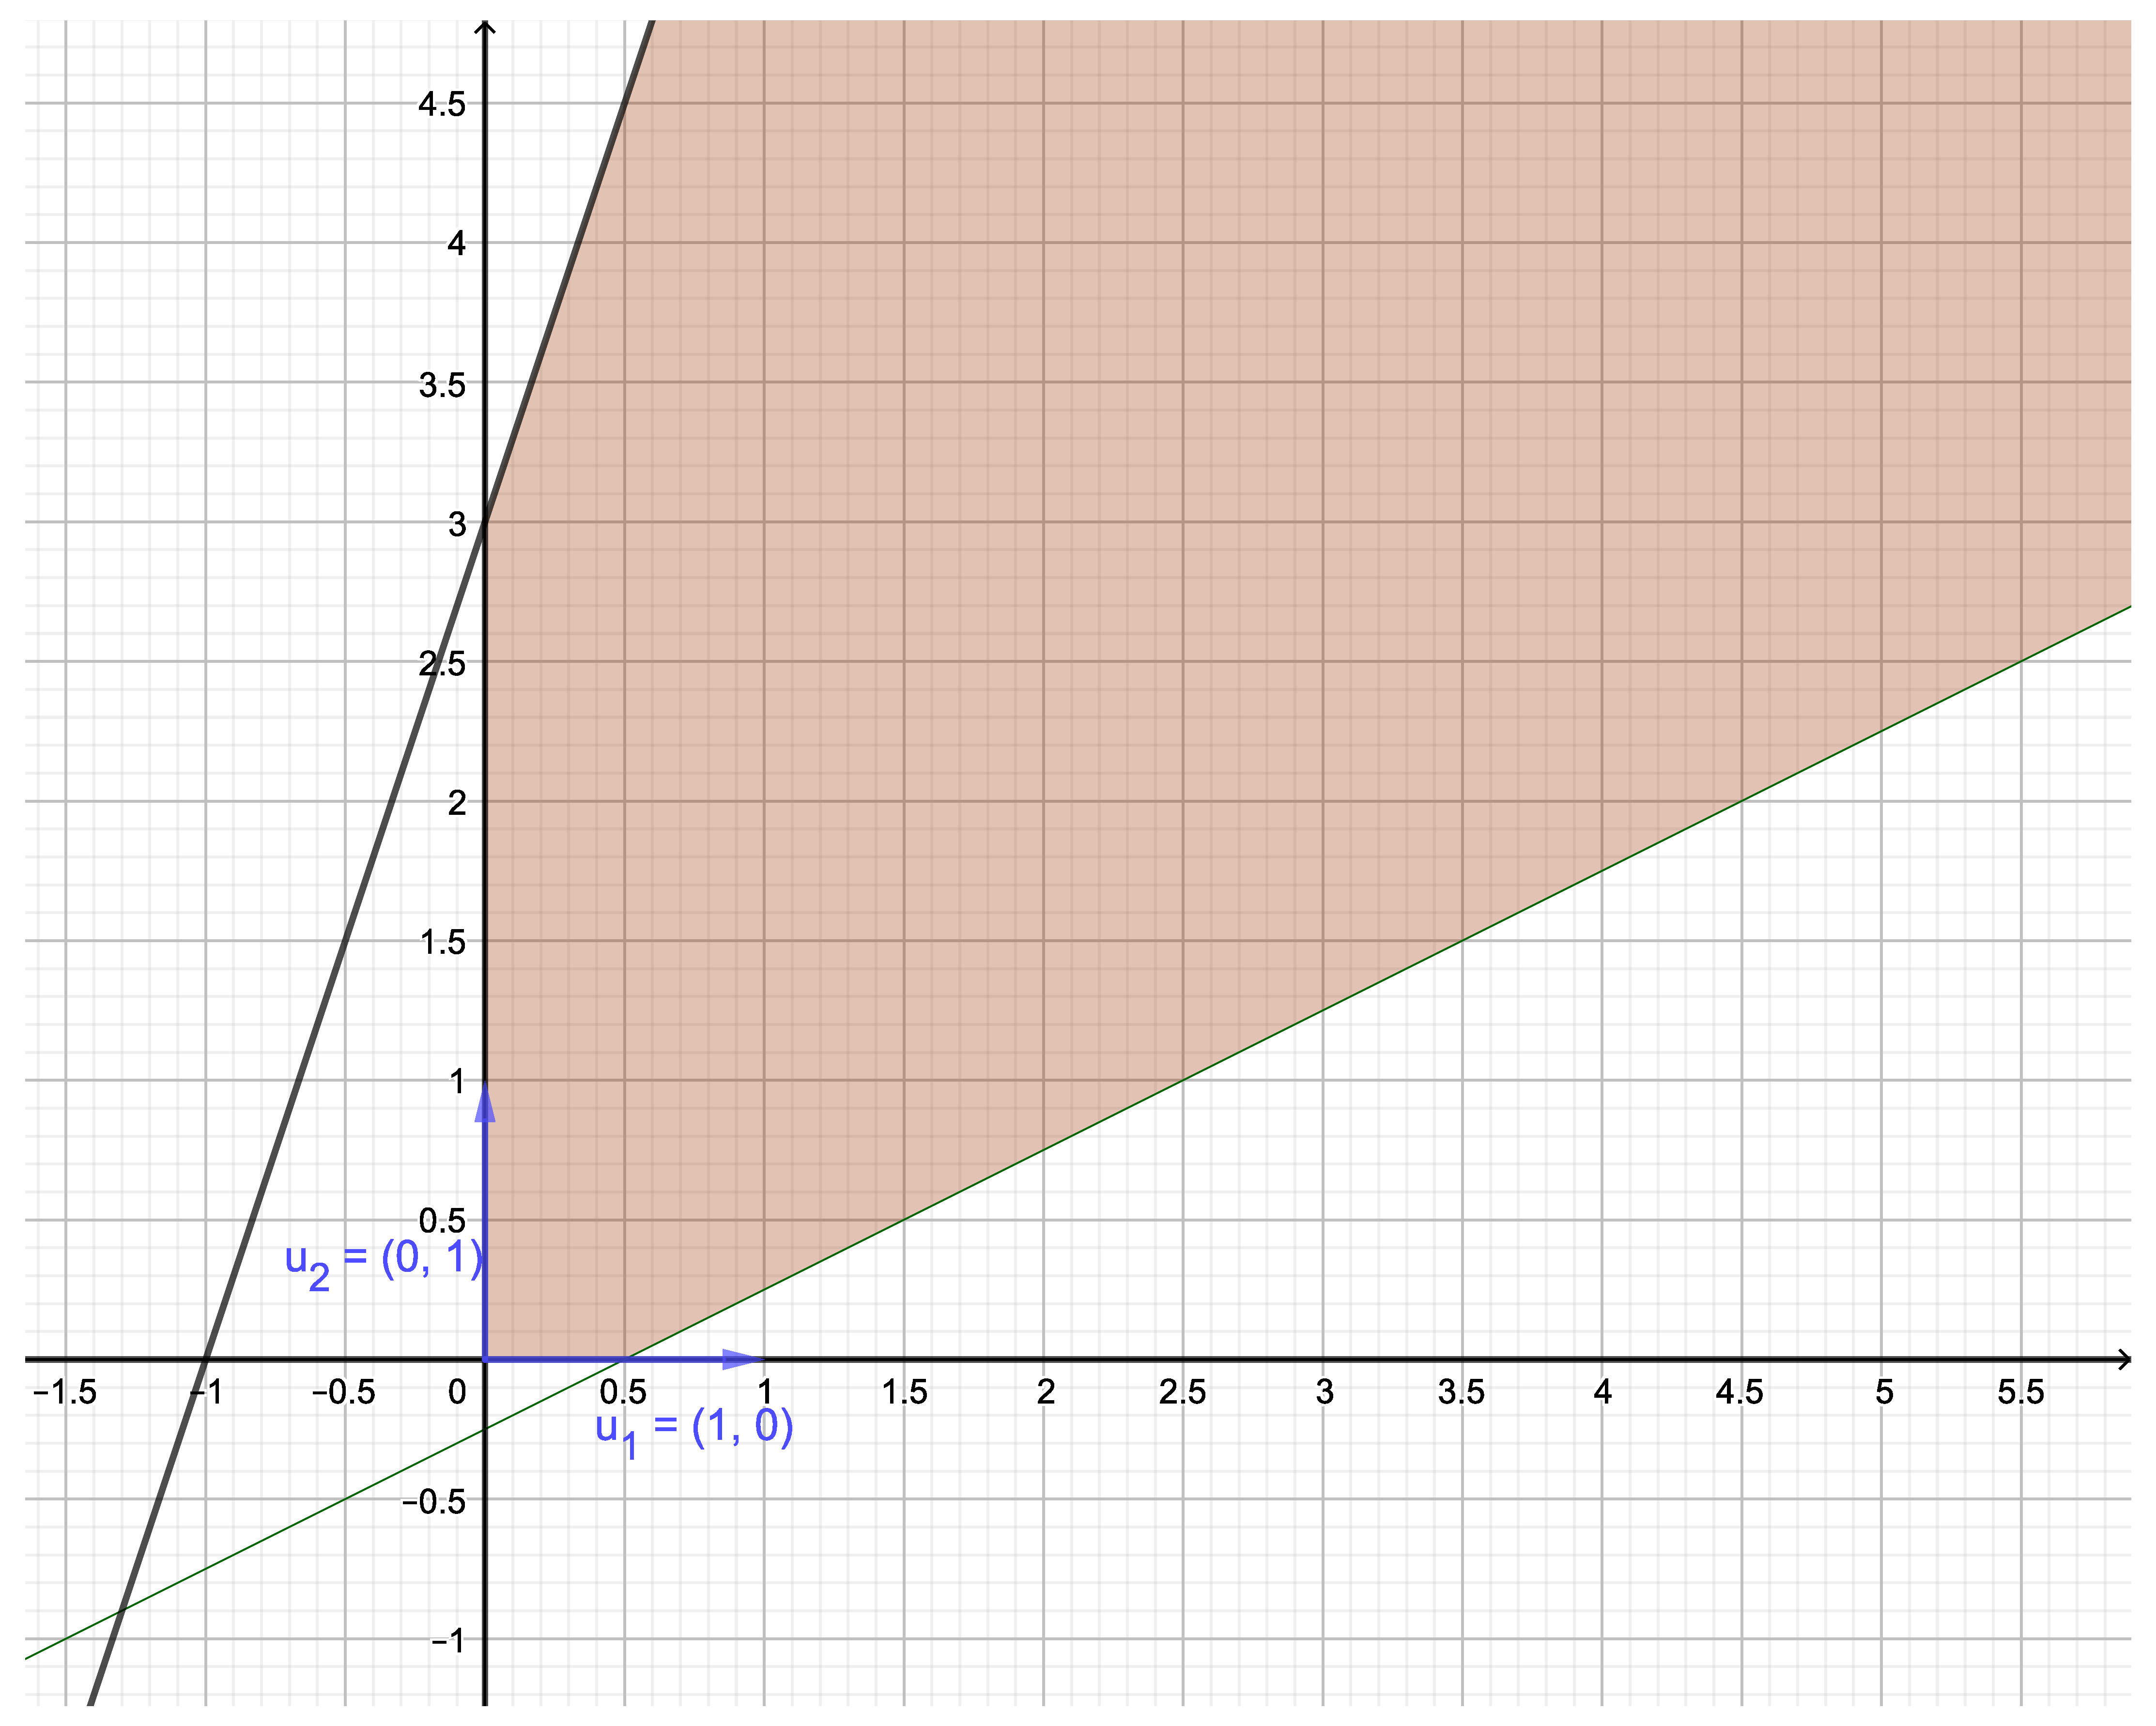
\includegraphics[width=0.5\textwidth]{p6.pdf}
\end{figure}

\FloatBarrier

\begin{enumerate}
\item [(a)]
Convert $P_1$ to standard equality form.
$$
\left\{
\begin{aligned}
& 2x_1 - 4x_2 + a_1 & & = 1 \\
& 3x_1 - x_2   & -a_2 & = -3 \\
& x_1, x_2, a_1, a_2 & & \geqslant 0.
\end{aligned}
\right.
$$

\item[(b)]
Basic solutions (in the form of $(x_1, x_2, a_1, a_2)$): 
$$
\begin{aligned}
&(-13/10, -9/10, 0, 0)   \\ 
&(-1, 0, 3, 0)\\ 
&(1/2, 0, 0, 9/2) \star\\
& (0, 3, 13, 0)\star\\ 
 &(0, -1/4, 0, 13/4)\\
 & (0, 0, 1, 3)\star
\end{aligned}
$$

\item[(c)]
Basic feasible solutions are those basic solutions with "$\star$".

\item[(d)]
Let $V$ be the set of all extremal directions. 
$$
V = \{v \in\mathbb R^2| v = (1, d)^T, d\in [1/2, 3] \}.
$$

\item[(e)]
From the figure, we can see that there are two moving directions to the adjacent points. $u_1$ is to point $(1/2, 0)^T$ and $u_2$ is to point $(0, 3)^T$.

$$
\begin{aligned}
&u_1 = (1, 0)^T \\
&u_2 = (0, 1)^T 
\end{aligned}
$$
\end{enumerate}

\section*{Problem 7}

We plot the region of $P_2$.

\begin{figure}[htbp]
  \caption{Region $P_2$.}
  \centering
    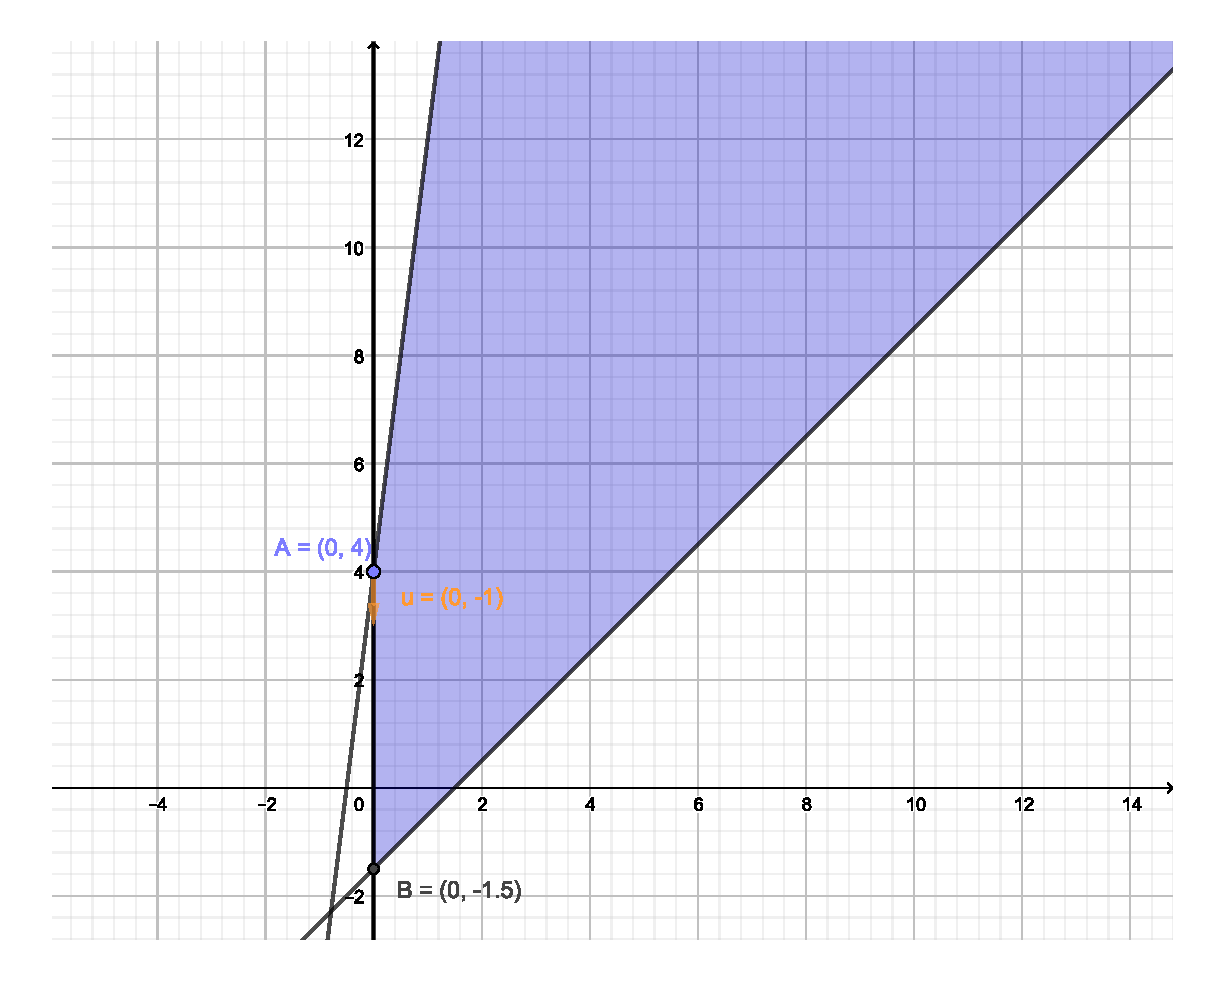
\includegraphics[width=0.5\textwidth]{p7.pdf}
\end{figure}

\FloatBarrier

\begin{enumerate}
\item [(a)]
Convert $P_2$ to standard equality form.
$$
\left\{
\begin{aligned}
& 2x_1 - 2x_2^+ + 2x_2^- + a_1 & & = 3 \\
& 8x_1 - x_2^+ + x_2^-   & -a_2 & = -4 \\
& x_1, x_2^+, x_2^-, a_1, a_2 & & \geqslant 0.
\end{aligned}
\right.
$$

\item[(b)]
Basic solutions (in the form of $(x_1, x_2^+, x_2^-, a_1, a_2)$): 
$$
\begin{aligned}
&(-1/2, -1, 0, 0, 0)   \\ 
&(-1/2, 1, 0, 0, 0) \\ 
&(-1/2, 0, 0, 4, 0) \\
& (3/2, 0, 0, 0, 16) \star \\ 
 &(0, 4, 0, 11, 0) \star \\
 & (0, -3/2, 0, 0, 11/2) \\
 & (0, 0, -4, 11, 0) \\
& (0, 0, 3/2, 0, 11/2) \star \\
& (0, 0, 0, 3, 4) \star
\end{aligned}
$$

\item[(c)]
Basic feasible solutions are those basic solutions with "$\star$".

\item[(d)]
Let $V$ be the set of all extremal directions. 
$$
V = \{v \in\mathbb R^2| v = (1, d)^T, d\in [1, 8] \}.
$$

\item[(e)]
From the figure, we can see that there is only one moving directions to the adjacent point $(0, -3/2)^T$. 

$$
u = (0, -1)^T
$$
\end{enumerate}

\end{document}